\section{clipbrecords.h File Reference}
\label{clipbrecords_8h}\index{clipbrecords.h@{clipbrecords.h}}
{\tt \#include $<$QWidget$>$}\par
{\tt \#include $<$QMime\-Data$>$}\par
{\tt \#include $<$QMap$>$}\par
{\tt \#include $<$QList$>$}\par


Include dependency graph for clipbrecords.h:\begin{figure}[H]
\begin{center}
\leavevmode
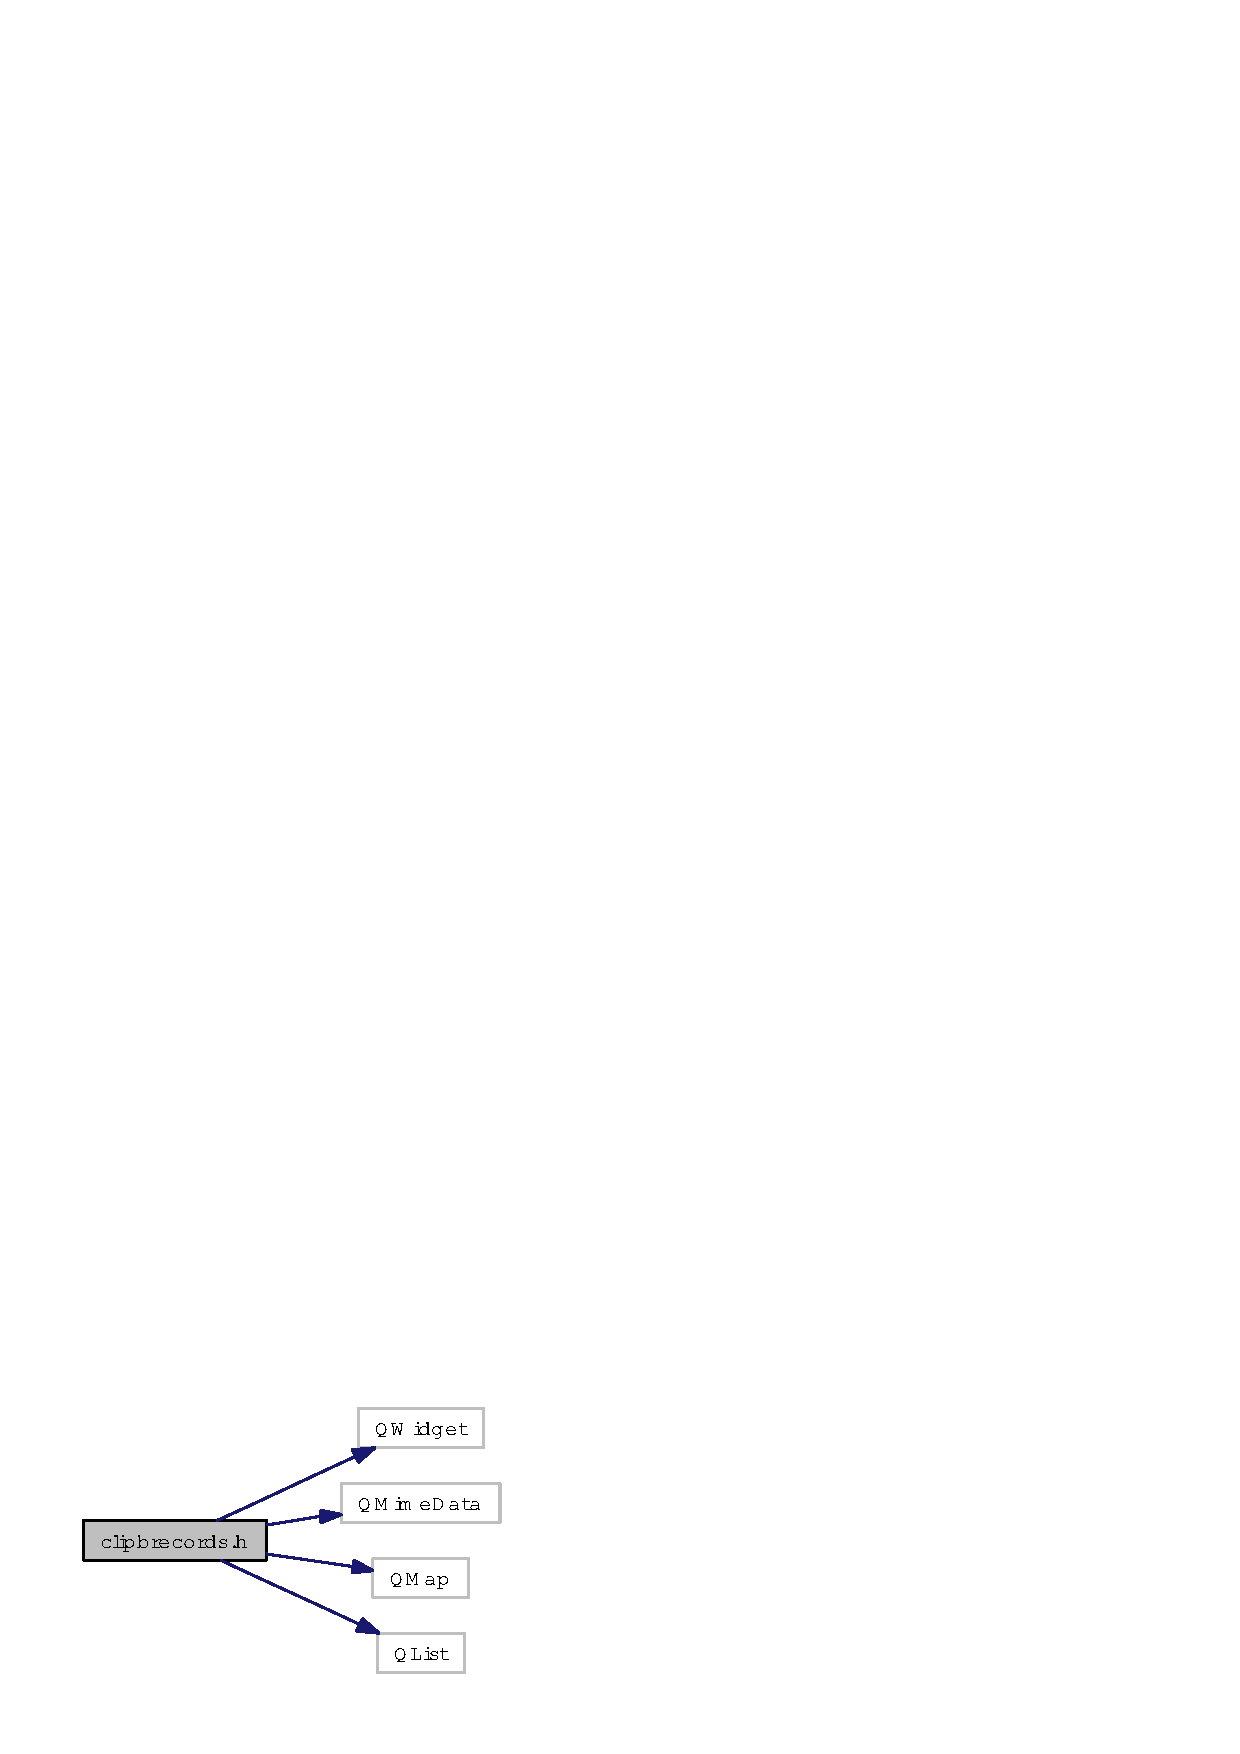
\includegraphics[width=122pt]{clipbrecords_8h__incl}
\end{center}
\end{figure}


This graph shows which files directly or indirectly include this file:\begin{figure}[H]
\begin{center}
\leavevmode
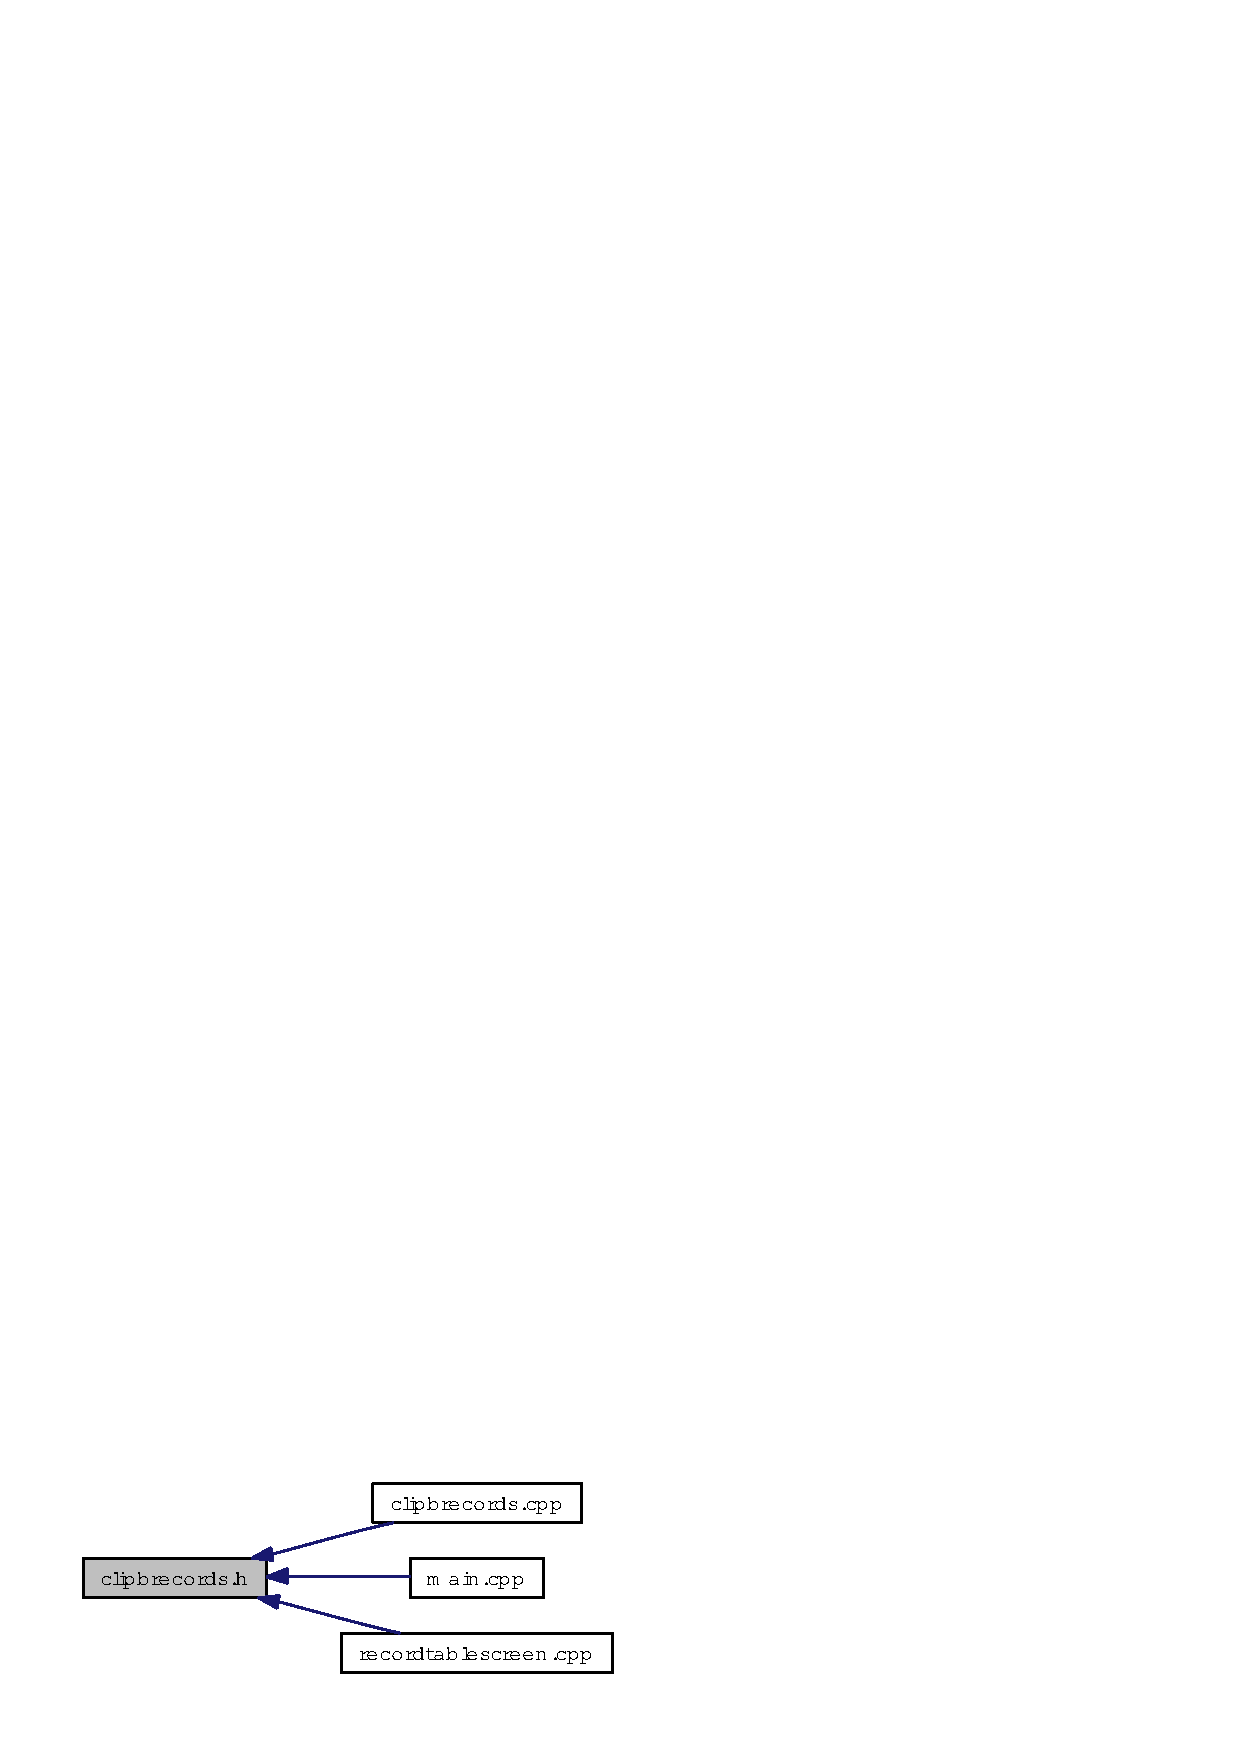
\includegraphics[width=149pt]{clipbrecords_8h__dep__incl}
\end{center}
\end{figure}
\subsection*{Classes}
\begin{CompactItemize}
\item 
struct {\bf clipb\_\-records\_\-struct}
\item 
class {\bf clipbrecords}
\end{CompactItemize}
\subsection*{Functions}
\begin{CompactItemize}
\item 
{\bf Q\_\-DECLARE\_\-METATYPE} ({\bf clipb\_\-records\_\-struct})
\end{CompactItemize}


\subsection{Function Documentation}
\index{clipbrecords.h@{clipbrecords.h}!Q_DECLARE_METATYPE@{Q\_\-DECLARE\_\-METATYPE}}
\index{Q_DECLARE_METATYPE@{Q\_\-DECLARE\_\-METATYPE}!clipbrecords.h@{clipbrecords.h}}
\subsubsection{\setlength{\rightskip}{0pt plus 5cm}Q\_\-DECLARE\_\-METATYPE ({\bf clipb\_\-records\_\-struct})}\label{clipbrecords_8h_5c1ec2e4882738887a0a2bd35e14ceb2}


